\subsection{Koordinateneinheitsvektoren und Standardbasis}
\label{subsec:vector_algebra_standard_basis}

Entlang jeder Koordinatenachse wird ein Einheitsvektor gewählt. Diese Vektoren
bilden das Grundgerüst der Koordinatendarstellung.

\begin{DefinitionBox}{Koordinateneinheitsvektoren}{vector_algebra_coordinate_unit_vectors}
  Die \emph{Koordinateneinheitsvektoren}
  \EnglishTerm{coordinate unit vectors} lauten
  \[
    \R^2:\quad
    \vec e_1=\begin{pmatrix}1\\0\end{pmatrix},
    \quad
    \vec e_2=\begin{pmatrix}0\\1\end{pmatrix},
  \]
  \[
    \R^3:\quad
    \vec e_1=\begin{pmatrix}1\\0\\0\end{pmatrix},
    \quad
    \vec e_2=\begin{pmatrix}0\\1\\0\end{pmatrix},
    \quad
    \vec e_3=\begin{pmatrix}0\\0\\1\end{pmatrix}.
  \]
  Sie stehen paarweise senkrecht aufeinander und bilden die
  \emph{Standardbasis} \EnglishTerm{standard basis}.
\end{DefinitionBox}

\begin{center}
  \CachedTikzFigure{content/resources/chapters/vector_algebra/tikz/standard_basis.tex}
\end{center}

\begin{RemarkBox}[title=Rechtssystem]
  \label{rem:vector_algebra_right_handed_system}
  Im $\R^3$ werden die Achsen üblicherweise als \emph{Rechtssystem}
  \EnglishTerm{right-handed coordinate system} orientiert. Die gekrümmte
  Orientierung von $\vec e_1$ nach $\vec e_2$ weist dabei in Richtung
  $\vec e_3$.
  \par\smallskip
  \noindent
  \begin{minipage}[c]{0.44\linewidth}
    \centering
    \CachedTikzFigure{content/resources/chapters/vector_algebra/tikz/right_handed_basis.tex}
  \end{minipage}\hfill
  \begin{minipage}[c]{0.50\linewidth}
    \centering
    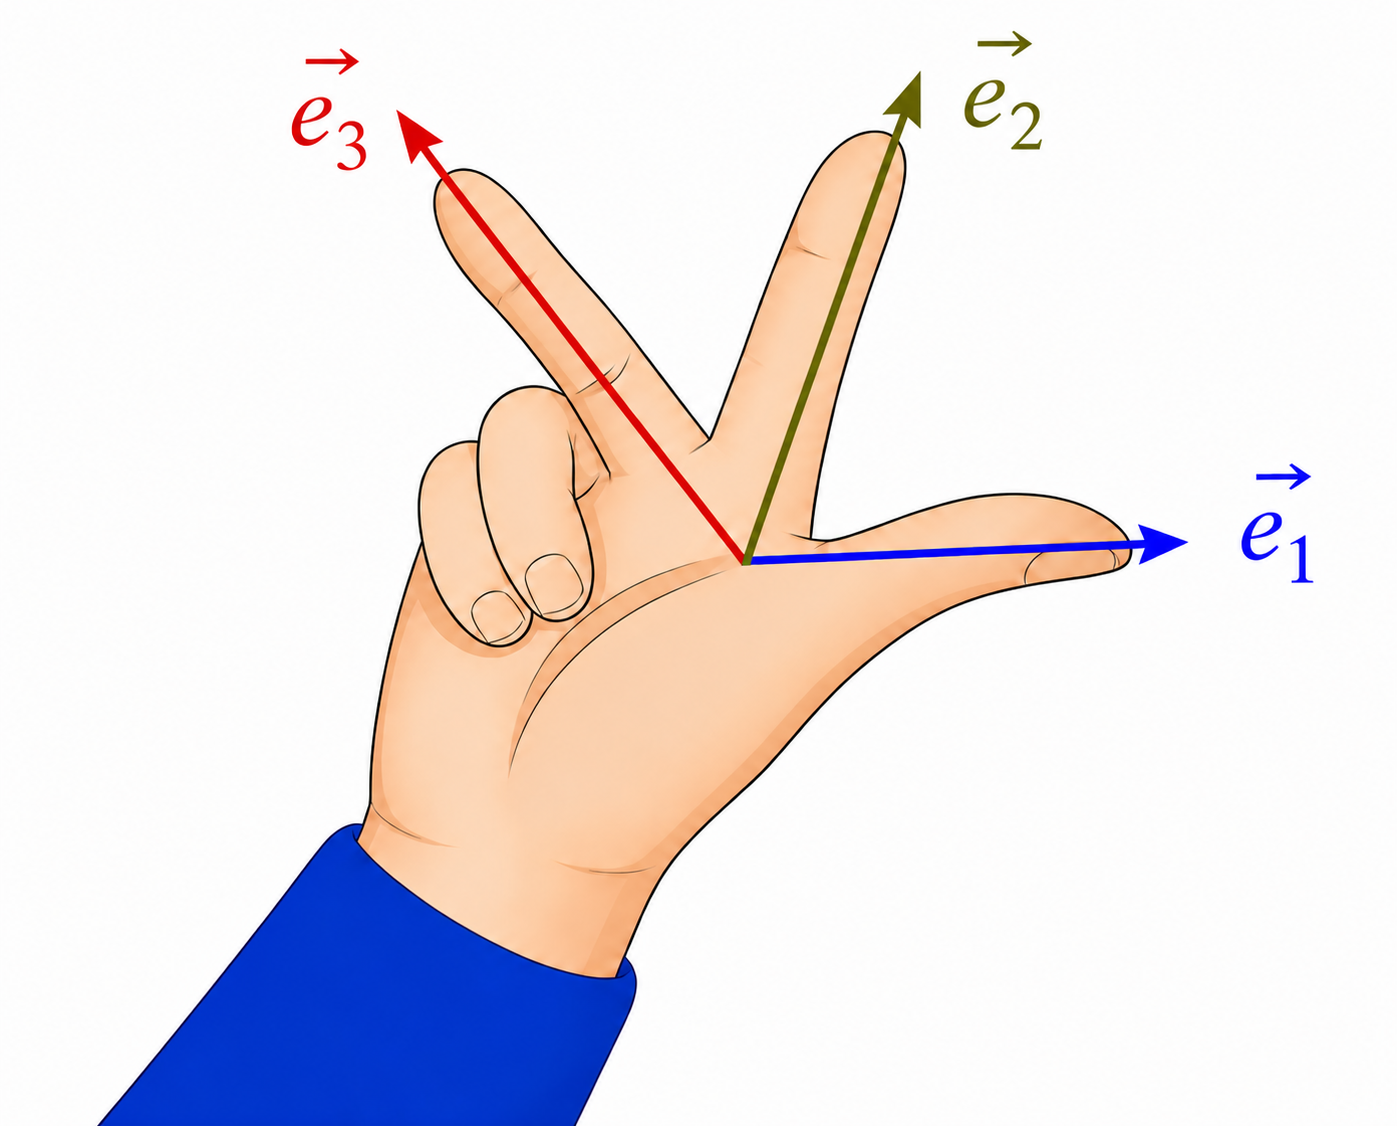
\includegraphics[width=0.68\linewidth]{content/resources/chapters/vector_algebra/images/right_handed_basis_hand.png}
  \end{minipage}
\end{RemarkBox}

\begin{KeyPointBox}{Darstellung in der Standardbasis}{vector_algebra_standard_basis_representation}
  Jeder Vektor ist die gewichtete Summe der Koordinateneinheitsvektoren:
  \[
    \R^2:\quad
    \begin{pmatrix}a_1\\a_2\end{pmatrix}
    =a_1\vec e_1+a_2\vec e_2,
    \qquad
    \R^3:\quad
    \begin{pmatrix}a_1\\a_2\\a_3\end{pmatrix}
    =a_1\vec e_1+a_2\vec e_2+a_3\vec e_3.
  \]
\end{KeyPointBox}

\begin{ExampleBox}{Koordinaten als Gewichte der Basisvektoren}{vector_algebra_basis_decomposition}
  \[
    \begin{pmatrix}2\\3\end{pmatrix}
    =\Cloze{6cm}{2\vec e_1+3\vec e_2},
    \qquad
    \begin{pmatrix}1\\2\\3\end{pmatrix}
    =\Cloze{8cm}{\vec e_1+2\vec e_2+3\vec e_3}.
  \]
\end{ExampleBox}
